\chapter{Stereo video watermarking}
\markright{Stereo video watermarking}
\label{wat}
\phantomsection
%\addcontentsline{toc}{chapter}{Stereoscopic Video}

\section{Watermaking}

Digital watermarking consists in imperceptiby and persistently associating some extra information with some original content. \\
The basic watermarking workflow is presented in Figure XX.\\
\begin{figure}[h!]
\centering
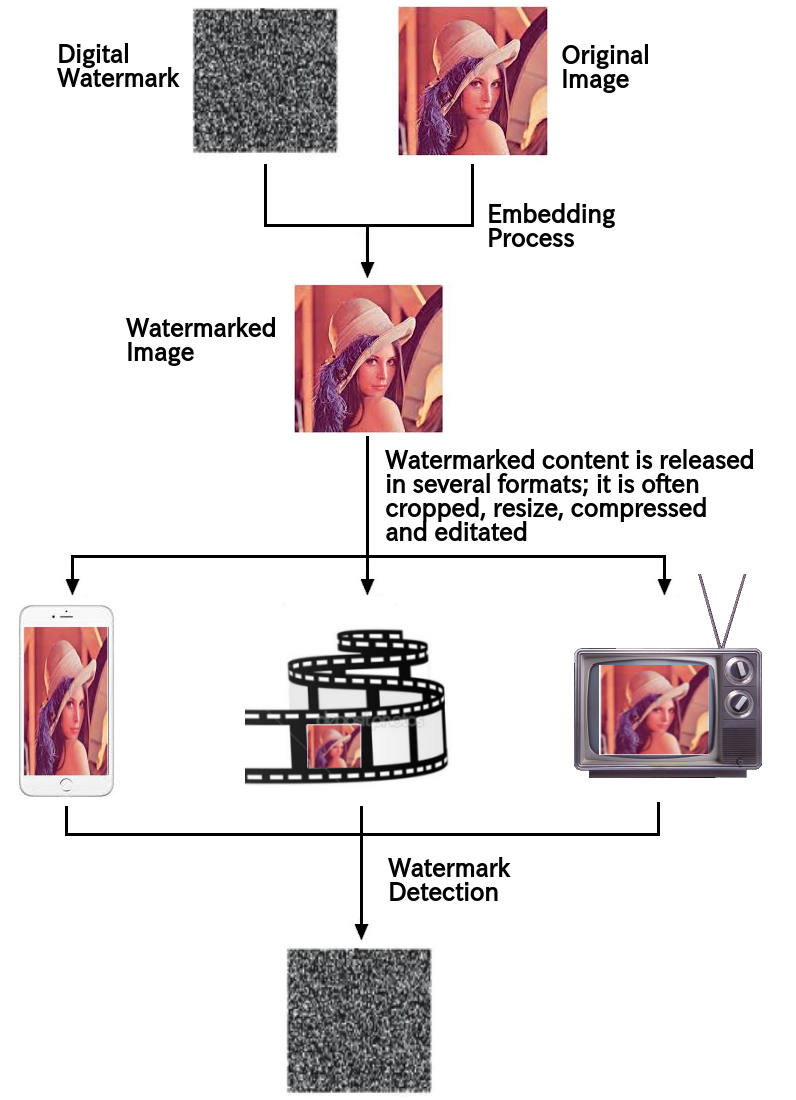
\includegraphics[width=0.3\textwidth]{./img/wat_workflow.png}
\caption{\small{Watermarking workflow}}
\label{fig:workflow}
\end{figure}
\newpage
\subsection{Properties}
Three parameters are required to evaluate watermarking technique performances:
\begin{itemize}
\item[-] transparency, that is the misure of how much the watermark affects the quality of the host data;
\item[-] robustness, i.e.,the capability of the hidden data to survive host signal manipulation including compression, signal processing, geometric manipulations;
\item[-] data payload, that is the amount of data of information bits that it is able to convey.
\end{itemize}
\begin{figure}[h!]
\centering
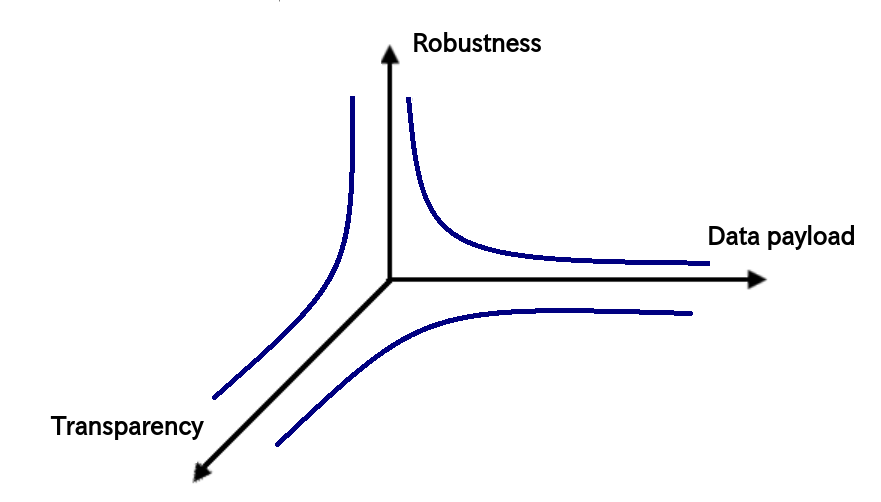
\includegraphics[width=0.4\textwidth]{./img/properties.png}
\caption{\small{Watermark properties trade-off}}
\label{fig:properties}
\end{figure}

\subsection{Embedding techniques}




\subsection{Embedding domains}


\section{Stereoscopic video watermarking}

\subsection{State of the art}



\newpage
In this thesis ....
due algoritmi di marchiatura presentati; il primo spaziale ss con rumore gaussiano etc.. 
il secondo ss nella frequenza additivo moltiplicativo...


data payload è ...
la trasparenza è stata valutata con ...
la robustezza è stata provata per view synthesis e compressione



